% Chapter 5

\chapter{Stochastische Galerkin-Methode}
\label{Chapter5}
Die stochastische Klein-Gordon-Gleichung wurde für eine $N$-dimensionale Zufallsvariable $Y$ und $y\in\R^N$ definiert durch
\begin{align}
\label{eqn:galerkin_skgg}
\partialdtt{u}(t,x,y)&=\alpha(y) \Laplace u(t,x,y) - \beta(x,\omega)u(t,x,y), \: t>0, \, x\in \Torus^d\\
u(0,x,y)&=g(x,y), \: x\in \Torus^d\nonumber\\
\partialdt{u}(0,x,y)&=h(x,y), \: x\in \Torus^d\nonumber
\end{align}
Seien $\Phi_m(Y)$ die zu $Y$ gehörenden gPC Basisfunktionen. Diese erfüllen die Orthogonalitätsbedingung 
\[\E[\Phi_i(Y)\Phi_j(Y)]=\delta_{ij}\] 
Sei $\Poly_P^N$ der Raum aller Polynome mit summiertem Grad kleiner gleich $P$ und Dimension $\binom{N+P}{P}$. Die gPC Projektion der Lösung der sKGG zu einem fixen Zeitpunkt $T>0$ und Ort $x\in\Torus^d$ ist definiert durch
\begin{align*}
u_M(T,x,Y)&=\sum_{m=0}^M\hat{u}_m(T,x)\Phi_m(Y)\in\Poly_P^N,\quad  M+1=\binom{N+P}{P}\\
\hat{u}_m(T,x)&=\E[u(T,x,Y)\Phi_m(Y)]
\end{align*}
Ist $\rho$ die Dichtefunktion von $Y$, so stimmt die gPC Projektion mit der Bestapproximation in $L_\rho^2$ überein. Diese Approximation ist im $L_\rho^2$ Sinne optimal, allerdings benötigen wir zur Berechnung der Koeffizienten $\hat{u}_m$ die unbekannte exakte Lösung $u(T,x,Y)$.\\
Der stochastische Galerkin Ansatz ist eine Erweiterung des klassischen Galerkin Ansatzes. Sei dazu eine weitere Approximation $v_M\in\Poly_P^N$ gegeben durch
\begin{equation}
v_M(t,x,Y)=\sum_{m=0}^M\hat{v}_m(t,x)\Phi_m(Y)
\end{equation}
Die Forderung an $v_M$ ist dann, dass das Residuum der sKGG (\ref{eqn:galerkin_skgg}) orthogonal zu allen Polynomen aus $\Poly_P^N$ ist. Eine Motivation dafür ist die schwache Lösung der sKGG, welche diese Orthogonalität für alle Polynome $\Poly^N$ erfüllt. Ist die schwache Lösung hinreichend regulär, so stimmt sie mit der Lösung der sKGG überein.
Konkret lautet die Orthogonalitätsbedingung an das Residuum für $t>0$ und $x\in\Torus^d$
\begin{equation}
\label{eqn:galerkinOrtho}
\E\left[\left(\partialdtt{v_M}(t,x,Y)-\alpha(Y)\Laplace v_M(t,x,Y)+\beta(x,Y)v_M(t,x,Y)\right)\Phi_k\right]=0
\end{equation} 
für alle $k=0,\dots,M$.\\
Wir wollen jetzt aus der Orthogonalitätsbedingung (\ref{eqn:galerkinOrtho}) eine Gleichung für die Koeffizienten $\hat{v}_m$ gewinnen. Dazu setzen wir die Definition von $v_M$ in die Gleichung ein und erhalten
\begin{align*}
\sum_{m=0}^M\partialdtt{\hat{v}}_m(t,x)\underbrace{\E[\Phi_m(Y)\Phi_k(Y)]}_{=\delta_{mk}}&=\E\left[\alpha(Y)\sum_{m=0}^M\Laplace \hat{v}_m(t,x)\Phi_m(Y)\Phi_k(Y)\right]\\
&\quad -\E\left[\beta(x,Y)\sum_{m=0}^M\hat{v}_m(t,x)\Phi_m(Y)\Phi_k(Y)\right]\\
\equivalent \qquad \partialdtt{\hat{v}}_k(t,x)&=\sum_{m=0}^M\Laplace \hat{v}_m(t,x)\underbrace{\E[\alpha(Y)\Phi_m(Y)\Phi_k(Y)]}_{=a_{mk}}\\
&\quad -\sum_{m=0}^M\hat{v}_m(t,x)\underbrace{\E[\beta(x,Y)\Phi_m(Y)\Phi_k(Y)]}_{=b_{mk}(x)}\\
\equivalent \qquad \partialdtt{\hat{v}}_k(t,x)&=a_k\Laplace \hat{v}(t,x)-b_k(x)\hat{v}(t,x)\\
\intertext{mit $ a_k=(a_{0k},\dots,a_{Mk}),\quad b_k(x)=(b_{0k}(x),\dots,b_{Mk}(x)),\quad \hat{v}(t,x)=(\hat{v}_0(t,x),\dots,\hat{v}_M(t,x))^T$}\\
\equivalent \qquad \partialdtt{\hat{v}}(t,x)&=A\Laplace \hat{v}(t,x)-B(x)\hat{v}(t,x)
\end{align*}
Die Matrizen $A$ und $B(x)$ werden durch die Zeilenvektoren $a_k$ und $b_k(x)$ gebildet und sind symmetrisch. Die benötigten Koeffizienten der Approximation $v_M$ sind gekoppelt und als Lösung folgender partieller Differentialgleichung zu erhalten
\begin{equation}
\label{eqn:galerkin_dgl}
\begin{split}
\partialdtt{\hat{v}}(t,x)&=A\Laplace \hat{v}(t,x)-B(x)\hat{v}(t,x)\\
\hat{v}(0,x)&=\hat{g}(x)\\
\partialdt{\hat{v}}(0,x)&=\hat{h}(x)\\
\end{split}
\end{equation}
Dabei gilt für die Anfangswerte $\hat{v}(0,x)$ und $\partialdt{\hat{v}}(0,x)$ wegen 
\[v_M(0,x,Y)=\sum_{m=0}^M\hat{v}_m(0,x)\Phi_m(Y)\]
und
\begin{align*}
g(x,y)&\approx v_M(0,x,y)\\
h(x,y)&\approx \partialdt{v}_M(0,x,y)
\end{align*}
die Darstellung mithilfe der Koeffizienten der Bestapproximation von $g$ und $h$
\begin{align*}
\hat{v}_m(0,x)=\hat{g}_m=\E[g(x,Y)\Phi_m(Y)]\\
\partialdt{\hat{v}}_m(0,x)=\hat{h}_m=\E[h(x,Y)\Phi_m(Y)]
\end{align*}
\section{Splitting für den Galerkin-Ansatz}
Die partielle Differentialgleichung (\ref{eqn:galerkin_dgl}) ist ein System mit Zeitableitung zweiter Ordnung und vektorwertig mit Größe $M+1$. Um eine numerische Lösung des Systems zu erhalten, bietet sich wieder ein Splitting-Ansatz an. Zuerst wollen wir das System aber so weit wie möglich entkoppeln.
\begin{maththeorem}
\label{th:galerkin_posdef}
Ist $\alpha(y)>c$ für ein $c>0$, so ist die Matrix $A$ aus dem Galerkin-Ansatz positiv definit und besitzt nur positive Eigenwerte $\lambda>c$.\\
Ist $\norm{\alpha}_\infty < \infty$, so gilt $\lambda\le \norm{\alpha}_\infty$.
\end{maththeorem}
\begin{proof}
Sei $z\in\R^{M+1}\setminus \lbrace 0\rbrace$ beliebig. Dann gilt wegen $a_{ij}=\int \alpha(y)\Phi_i(y)\Phi_j(y)\rho(y)dy$
\[(Az)_i=\int \alpha(y)\Phi_i(y)\underbrace{\left(\sum_{j=0}^M\Phi_j(y)z_j\right)}_{=\tilde{z}(y)}\rho(y)dy\]
und daher
\begin{align*}
z^TAz&=\int \alpha(y)\left(\sum_{i=0}^M\Phi_i(y)z_i\right)\tilde{z}(y)\rho(y)dy\\
&=\int\underbrace{\alpha(y)}_{>c}\underbrace{\tilde{z}^2(y)}_{>0 \text{ f.ü.}}\underbrace{\rho(y)}_{>0}dy\\
&>c\int \tilde{z}^2(y)\rho(y)dy\\
&=c\sum_{i=0}^Mz_i\sum_{j=0}^Mz_j\underbrace{\int \Phi_i(y)\Phi_j(y)\rho(y)dy}_{=\delta_{ij}}\\
&=cz^Tz
\end{align*}
Die Abschätzung nach oben ergibt sich ähnlich, da für einen Eigenvektor $z\neq 0$ zum Eigenwert $\lambda$ gilt
\[|\lambda| z^Tz=|z^TAz|=\left|\int \alpha(y)\tilde{z}^2(y)\rho(y)dy\right|\leq \norm{\alpha}_\infty z^Tz\]
\end{proof}
Unter entsprechenden Voraussetzungen an $\beta(x,y)$ gelten die Aussagen von Satz \ref{th:galerkin_posdef} punktweise auch für $B(x)$.
\subsection{Entkopplung des ersten Teils}
Wir können $A\in\R^{M+1\times M+1}$ zerlegen in
\[A=S_1D_1S_1^T,\quad \text{$D_1$ diagonal und $S_1$ orthogonal}\]
Wir definieren dann 
\[w(t,x)\coloneqq S_1^T\hat{v}(t,x),\quad t>0,x\in\Torus^d\]
und schreiben das System (\ref{eqn:galerkin_dgl}) in der Form
\begin{equation}
\label{eqn:galerkin_dgl_transformed}
\begin{split}
\partialdtt{w}(t,x)&=D_1\Laplace w(t,x)-S_1^TB(x)S_1w(t,x)\\
w(0,x)&=S_1^T\hat{g}(x)\\
\partialdt{w}(0,x)&=S_1^T\hat{h}(x)\\
\end{split}
\end{equation}
Schreiben wir es anschließend formal um in ein System mit Zeitableitung erster Ordnung, so gilt für $\tilde{w}\coloneqq \partialdt w$ und ein Gewicht $\kappa\in[0,1]$
\[\partialdt\begin{pmatrix}w\\ \tilde{w}\end{pmatrix}(t,x)=\left[\begin{pmatrix}0 & \kappa I_{M+1}\\ D_1\Laplace& 0\end{pmatrix}+\begin{pmatrix}0&(1-\kappa)I_{M+1}\\-S_1^TB(x)S_1 & 0\end{pmatrix}\right]
\begin{pmatrix}w\\\tilde{w}\end{pmatrix}(t,x)\]
Das Splitting besteht dann aus den zwei Gleichungen
\begin{equation}
\label{eqn:galerkin_split1}
\partialdt\begin{pmatrix}w_1\\ \tilde{w}_1\end{pmatrix}(t,x)=\begin{pmatrix}0 & \kappa I_{M+1}\\ D_1\Laplace& 0\end{pmatrix}\begin{pmatrix}w_1\\\tilde{w}_1\end{pmatrix}(t,x)
\end{equation}
und
\begin{equation}
\label{eqn:galerkin_split2}
\partialdt\begin{pmatrix}w_2\\ \tilde{w}_2\end{pmatrix}(t,x)=\begin{pmatrix}0&(1-\kappa)I_{M+1}\\-S_1^TB(x)S_1 & 0\end{pmatrix}\begin{pmatrix}w_2\\\tilde{w}_2\end{pmatrix}(t,x)
\end{equation}
Diese sind wie schon in Kapitel \ref{chapter:solver_kgg} mithilfe der Matrixexponentialfunktion lösbar. Beachte, dass die Gleichung (\ref{eqn:galerkin_split1}) nach Umsortierung in $2\times 2$ Systeme entkoppelt ist, da $D_1$ diagonal ist. Die Matrixexponentialfunktion der entkoppelten $2\times 2$ Systeme ist in Algorithmus \ref{alg:kgg_solver} als \emph{First\_Part\_Solver} in einfacher Darstellung direkt gegeben. Der erste Teil des Splittings besteht somit aus dem Lösen von $M+1$ unabhängigen "'Wellengleichungen"' (Name passend für $\kappa=1$). Die Eigenwerte $d_i$ von $A$ sind die Quadrate der Wellengeschwindigkeiten. Abschätzungen für diese, insbesondere Positivität, erhalten wir mithilfe von Satz \ref{th:galerkin_posdef} unter entsprechenden Voraussetzungen an $\alpha(y)$.

\subsection{Entkopplung des zweiten Teils}
Analog zum ersten Teil können wir für jedes fixe $x\in\Torus^d$ die symmetrische Matrix $S_1^TB(x)S_1\in\R^{M+1\times M+1}$ zerlegen in $S_1^TB(x)S_1=S_2(x)D_2(x)S_2^T(x)$ mit $S_2(x)$ orthonormal und $D_2(x)$ diagonal.\\
Definiere
\[z(t,x)\coloneqq S_2^T(x) w_2(t,x), \quad \tilde{z}(t,x)=\partialdt{z}(t,x)\]
Dann ist (\ref{eqn:galerkin_split2}) äquivalent zum System
\begin{equation}
\label{eqn:galerkin_split2_decoup}
\partialdt\begin{pmatrix}z\\ \tilde{z}\end{pmatrix}(t,x)=\begin{pmatrix}0&(1-\kappa)I_{M+1}\\-D_2(x) & 0\end{pmatrix}\begin{pmatrix}z\\\tilde{z}\end{pmatrix}(t,x)
\end{equation}
Das System (\ref{eqn:galerkin_split2_decoup}) ist nach Umsortierung in $2\times 2$ Blöcke entkoppelt. Die Matrixexponentialfunktion dieser Blöcke können wir mit der Funktion \emph{Second\_Part\_Solver} aus Algorithmus \ref{alg:kgg_solver} effizient lösen. Der große Vorteil hierbei ist, dass die Berechnung der Matrixexponentialfunktion der $2M+2\times 2M+2$ Matrix aus (\ref{eqn:galerkin_split2}) für jedes $x$ im Gitter entfällt. Der Trade-off ist, dass in jedem Splittingschritt die Transformation und Rücktransformation mit $S_2(x)$ durchgeführt werden muss. Dieser zusätzliche Aufwand fällt jedoch im Gegensatz zur teuren Matrixexponentialfunktion, welche die Blockstruktur der Matrix nicht berücksichtigt, nicht stark ins Gewicht.
\subsection{Algorithmus}
In Algorithmus \ref{alg:galerkin} ist die Vorgehensweise für den Galerkin-Ansatz zum Lösen der stochastischen KGG skizziert. Als Basis dienen dabei die Kernfunktionen des allgemeinen KGG Lösers aus Algorithmus \ref{alg:kgg_solver}, welche in einem schnellen Strang-Splitting eingebettet sind.
\begin{algorithm}[ht]
    \caption{Galerkin für die stochastische KGG.}
    \label{alg:galerkin}
    \begin{algorithmic}[1] % The number tells where the line numbering should start
        \Function{Galerkin}{$H, u_0, v_0, \alpha,\beta,\kappa,Y, M,\tau, T$} 
            	\State $\Phi_m\gets$ $m$-te orthonormale gPC-Basis-Funktion zu $Y$, $\quad m=0,\dots,M$
              \State $A_{mk}\gets \E[\alpha(Y)\Phi_m(Y)\Phi_k(Y)],\quad m,k=0,\dots,M$
              \State $A=S_1D_1S_1^T, \quad S_1$ orthonormal, $D_1$ diagonal
              \State $x_H\gets$ Ortsdiskretisierung der Größe $H$
              \For{$x\in x_H$}
              	\State $B_{mk}(x)\gets \E[\beta(x,Y)\Phi_m(Y)\Phi_k(Y)],\quad m,k=0,\dots,M$
              	\State $S_1^TB(x)S_1=S_2(x)D_2(x)S_2^T(x)$, $S_2(x)$ orthonormal, $D_2(x)$ diagonal
              \EndFor
              \State
              \LineComment{FastStrang Splitting für entkoppelte Systeme:}
              \State $g\gets S_1^T\cdot (\E[u_0(x_H,Y)\Phi_m(Y)])_{m=0,\dots,M}$
              \State $h\gets S_1^T\cdot (\E[v_0(x_H,Y)\Phi_m(Y)])_{m=0,\dots,M}$
              \State $g,h\gets \text{Multi\_First\_Part\_Solver}(H, g, h, \diag(D_1), \kappa, \frac{\tau}{2})$
            \State $g,h\gets \text{Multi\_Second\_Part\_Solver}(x_H, g, h, \diag(D_2), S_2, 1-\kappa, \tau)$
            \For{$i=1,\dots,\frac{T}{\tau}-1$} \Comment{Annahme: $\frac{T}{\tau}\in\N$} 
            	\State $g,h\gets \text{Multi\_First\_Part\_Solver}(H, g, h, \diag(D_1), \kappa, \tau)$
            \State $g,h\gets \text{Multi\_Second\_Part\_Solver}(x_H, g, h, \diag(D_2), S_2, 1-\kappa, \tau)$
            \EndFor
            \State $g,h\gets \text{Multi\_First\_Part\_Solver}(H, g, h, \diag(D_1), \kappa, \frac{\tau}{2})$
            \State
            \LineComment{Rücktransformation und Extraktion der Statistiken:}
            \State $\hat{v}\gets S_1g$  
            \State $\mu\gets \hat{v}_{0,j=1,\dots,H}$ 
			\State $\sigma^2_j\gets \sum_{m=1,\dots,M}\hat{v}^2_{mj}$
			\State \textbf{return} $\mu,\sigma^2$
        \EndFunction
        \Function{Multi\_First\_Part\_Solver}{$H, g, h, \alpha, \kappa, \tau$}
        	\For{$i=0,\dots,M$}
        		\State $\tilde{g}_i,\tilde{h}_i\gets \text{First\_Part\_Solver}(H,g_i, h_i,\alpha_i,\kappa,\tau)$
        	\EndFor
        	\State \textbf{return} $(\tilde{g}_0,\dots,\tilde{g}_M)^T, (\tilde{h}_0,\dots,\tilde{h}_M)^T$
        \EndFunction
        \Function{Multi\_Second\_Part\_Solver}{$x_H,g,h,\beta,S_2,\tilde{\kappa},\tau$}
        	\State $g,h\gets S_2^T(x_H)g, S_2^T(x_H)h$
        	\For{$i=0,\dots,M$}
        		\State $\tilde{g}_i,\tilde{h}_i\gets \text{Second\_Part\_Solver}(x_H,g_i,h_i,\beta_i,\tilde{\kappa},\tau)$
        	\EndFor
        	\State \textbf{return} $S_2(x_H)\cdot (\tilde{g}_0,\dots,\tilde{g}_M)^T, S_2(x_H)\cdot (\tilde{h}_0,\dots,\tilde{h}_M)^T$
        \EndFunction
        
    \end{algorithmic}
\end{algorithm}
\subsubsection*{Berechnung der Erwartungswerte}
Die auftretenden Erwartungswerte zur Berechnung von $A$, $B(x)$, $g$ und $h$ können numerisch mithilfe von Quadraturformeln gelöst werden können. Mögliche Varianten wurden --insbesondere auch für mehrdimensionale Quadratur-- in Kapitel \ref{sec:discrete_proj} vorgestellt.\\
Sind $\alpha$, $\beta$ und die Anfangswerte glatte Funktionen, so bietet sich die Verwendung der Gauss-Quadratur an. Diese besitzt eine hohe polynomiale Exaktheit und berücksichtigt die Wahrscheinlichkeitsdichten implizit. Da die benötigten Stützstellen und ihre Anzahl feststehen, ist der Zeitaufwand dieser Quadratur im Vorhinein bekannt und vergleichsweise gering.\\[0.2cm]
Sind die Funktionen nicht glatt und besitzen beispielsweise Unstetigkeitsstellen, so bietet sich die Verwendung eines general-purpose Integrators an. Beachte, dass dieser die Wahrscheinlichkeitsdichten von $Y$ explizit auswerten muss. Diese Integratoren werden von verschiedenen Bibliotheken zur Verfügung gestellt und versuchen unter anderem Intervalle anhand der Unstetigkeitsstellen zu unterteilen. Dafür werden deutlich mehr Funktionsauswertungen benötigt und der Zeitaufwand lässt sich bei solchen Black-Box-Algorithmen nicht im Vorhinein bestimmen. Im Gegensatz zur Kollokation mithilfe von diskreter Projektion, wo eine Funktionsauswertung das Lösen einer Instanz der KGG entsprach, ist es hier jedoch möglich, die zu integrierende Funktion schnell und für beliebige $y\in\R^N$ auszuwerten.\\[0.2cm]
Weiterhin sei bemerkt, dass die Berechnungen der Erwartungswerte einmalig am Anfang passieren und unabhängig von der Stoppzeit $T$ sind. Variiert man die Polynomgrenze $P$, so kann man bereits berechnete Koeffizienten entsprechend wiederverwenden.
\section{Numerische Ergebnisse}
\subsection{Einfluss der Zeitschrittweite $\tau$}
Anhand der vierdimensionalen \nameref{trial:8} beobachten wir für verschiedene Werte von $P$ mit $M=\binom{4+P}{P}$ Polynomen den Einfluss der Zeitschrittweite $\tau$ auf die Approximationsgenauigkeit. Dieser Einfluss ist in Abbildung \ref{fig:galerkin_bydt_trial8} durch den Fehler des Erwartungswerts und der Varianz dargestellt. Wir erkennen, dass für $P\le 5$ die Wahl $\tau=10^{-3}$ ausreichend ist für eine bestmögliche Approximation. Der Fehler konvergiert quadratisch bezüglich des Parameters $\tau$, der bestmögliche Fehler ist aber durch den Parameter $P$ eingeschränkt und die Konvergenz endet vorzeitig.\\
Für $P=5$ ist $M=126$ und es steckt bereits ein großer Aufwand darin, die Matrizen $B(x)$ der Größe $126\times 126$ für jeden der 128 Knotenpunkte $x\in\Torus$ zu berechnen, da jeweils eine dünne Gitter Quadratur mit 9065 Punkten verwendet werden muss.
\begin{figure}
\centering
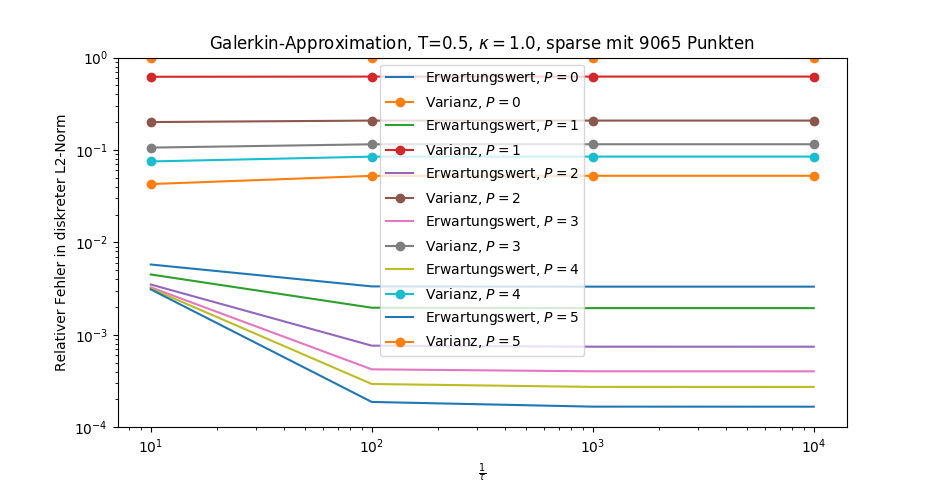
\includegraphics[width=\textwidth]{Figures/galerkin_trial8_sparse.png}
\caption{Fehler der Galerkin-Approximation von \nameref{trial:8} anhand von der für das Strang-Splitting verwendeten Zeitschrittweite $\tau$.}
\label{fig:galerkin_bydt_trial8}
\end{figure}

\subsection{Einfluss des Quadraturfehlers}
Wie bereits bei der Kollokation betrachten wir wieder die \nameref{trial:discontsimple} mit unstetigen Koeffizienten $\alpha$ und $\beta$. In Abbildung \ref{fig:galerkin_bydegree_trialdiscontsimple} ist der Fehler der Approximationen in Abhängigkeit vom Polynomgrad $P$ dargestellt. Der linke Plot erinnert an das Verhalten der Approximation mithilfe von Kollokation mithilfe von diskreter Projektion. Die dort verwendete Quadratur verwendet als Stützstellen Lösungen der deterministischen KGG. Dies macht einen general-purpose Integrator unpraktikabel. Hier jedoch erkennen wir, dass es möglich ist einen monoton fallenden Fehler zu erhalten, wenn die Berechnung von $A$ und $B(x)$ exakt ist. 
\begin{figure}[!htb]
\minipage{0.5\textwidth}
  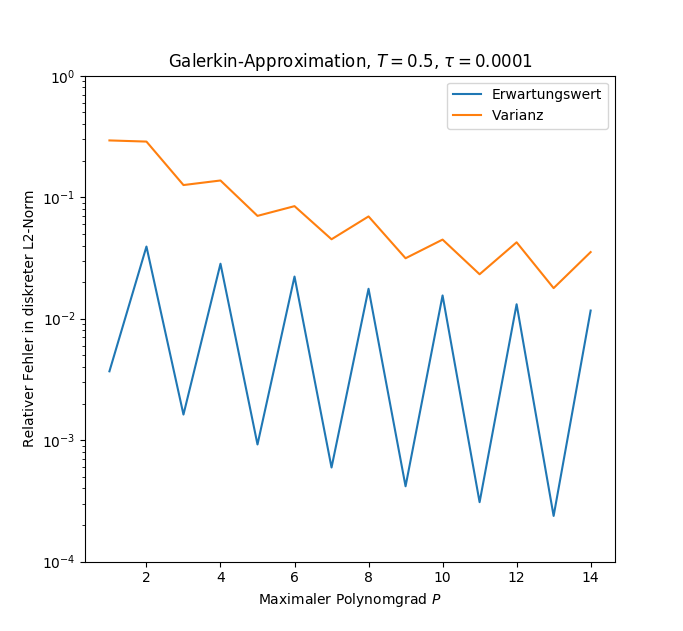
\includegraphics[width=\linewidth]{Figures/galerkin_bydegree_trialsimple_gauss.png}
\endminipage
\minipage{0.5\textwidth}
  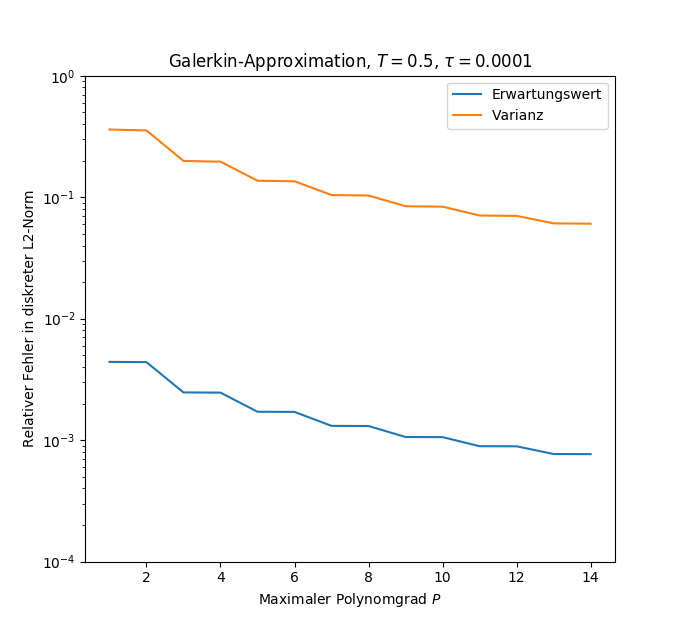
\includegraphics[width=\linewidth]{Figures/galerkin_bydegree_trial_simple_genpurp.png}
\endminipage
  \caption{Galerkin Approximation von \nameref{trial:discontsimple}. Links mit Gauss-Quadratur, rechts mit einem general-purpose Integrator.}
  \label{fig:galerkin_bydegree_trialdiscontsimple}
\end{figure}
\newline
Eine ähnliche Beobachtung machen wir auch für die \nameref{trial:disconttriple} mit 2 Unstetigkeitsstellen in $\alpha$ und stetigem $\beta$ in Abbildung \ref{fig:galerkin_bydegree_trialtriple}. Im Gegensatz zur Kollokation die einfache Möglichkeit einen monoton fallenden Fehler zu erhalten ohne große Laufzeitprobleme.
 \begin{figure}[!htb]
\minipage{0.5\textwidth}
  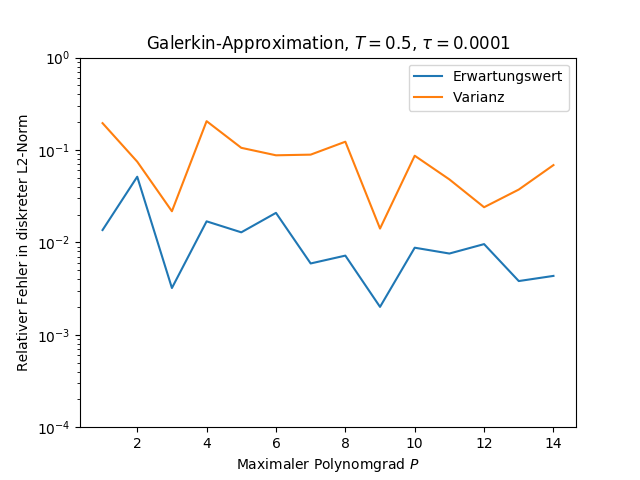
\includegraphics[width=\linewidth]{Figures/galerkin_bydegree_trialdisconttriple_gauss.png}
\endminipage
\minipage{0.5\textwidth}
  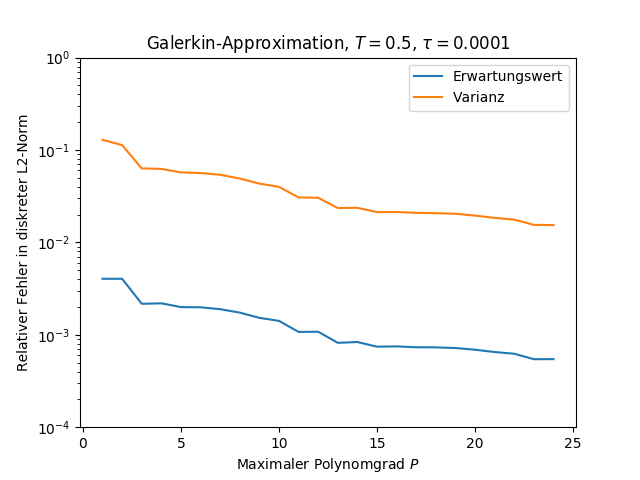
\includegraphics[width=\linewidth]{Figures/galerkin_bydegree_trialdisconttriple_genpurp.png}
\endminipage
  \caption{Galerkin Approximation von \nameref{trial:disconttriple}. Links mit Gauss-Quadratur, rechts mit einem general-purpose Integrator.}
  \label{fig:galerkin_bydegree_trialtriple}
\end{figure}
\subsection{Einfluss der Stoppzeit}
\begin{maththeorem}[Adaption von Theorem 2.2 aus \autocite{davidgottliebdongbinxiu2008}]
\label{th:adapted22}
Ziel: Abschätzung für 
\begin{align*}
\E\left[\norm{u-v_M}_2^2\right]&=\E\left[\int_{-\pi}^{\pi}\left(u(t,x,Y)-v_M(t,x,Y)\right)^2dx\right]\\
&=\int_{-\pi}^\pi\norm{u(t,x,y)-v_M(t,x,y)}_{L_\rho^2}^2dx\\
&\stackrel{\text{Parseval}}{=}\int_{-\pi}^\pi\sum_{m=0}^\infty |\langle u(t,x,y)-v_M(t,x,y),\Phi_m(y)\rangle_{L_\rho^2}|^2dx\\
&=\int_{-\pi}^\pi\sum_{m=0}^\infty\left(\hat{u}_m(t,x)-\hat{v}_m(t,x)\right)^2dx,\quad \hat{v}_m=0 \text{ für } m>M\\
&=\sum_{m=0}^\infty\norm{\hat{u}_m-\hat{v}_m}_2^2\\
&\le \sum_{m=0}^M\norm{\hat{u}_m-\hat{v}_m}_2^2 + \sum_{m=M+1}^\infty \frac{K}{m^{2\ell}}
\end{align*}
\todo[inline]{Problem1: In Vorlage geht Summe nur bis $M$, nicht unendlich.}
\todo[inline]{Problem2: In Vorlage gibt es Voraussetzung 
\[\norm{\hat{u}_m}_2^2\le \norm{\hat{u}_m}_1^2=\int_{-\pi}^\pi\left(\hat{u}^2_m+\left(\dx{\hat{u}_m}\right)^2\right)dx\le \frac{K}{m^{2\ell}},\quad K,\ell>0, m \text{ groß}.\]
Zusammen mit der Summe bis unendlich würde dies einen weiteren Term $\sum_{m=M+1}^\infty \frac{K}{m^{2\ell}}$ auf der rechten Seite der Gesamtabschätzung ergeben. Für $\ell\le\onehalf$ wäre diese Reihe nicht mal konvergent. Wie kommt es, dass dieser Term beim Autor nicht auftaucht?}
\end{maththeorem}
\begin{proof}[Beweisideen]
Sei 
\[e_m(t,x)\coloneqq \hat{u}_m(t,x)-\hat{v}_m(t,x),\quad m=0,\dots,M\]
Verwenden wir den Galerkin-Ansatz (\ref{eqn:galerkinOrtho}) für die Reihendarstellung von $u$ anstelle von $v_M$, so erhalten wir analog zum Ergebnis für $v_M$ die Gleichungen
\begin{equation}
\partialdtt{\hat{u}}_k(t,x)=\sum_{m=0}^\infty \Laplace \hat{u}_m(t,x)a_{mk}-\sum_{m=0}^\infty \hat{u}_m(t,x)b_{mk}(x),\quad k=0,\dots,M
\end{equation}
Subtrahieren wir davon die Gleichungen
\begin{equation}
\partialdtt{\hat{v}}_k(t,x)=\sum_{m=0}^M\Laplace \hat{v}_m(t,x)a_{mk}-\sum_{m=0}^M\hat{v}_m(t,x)b_{mk}(x),\quad k=0,\dots,M
\end{equation}
so erhalten wir für $k=0,\dots,M$
\begin{equation}
\label{eqn:error_eq_1}
\begin{split}
\partialdtt{e_k}(t,x)&=\sum_{m=0}^M\Laplace e_m(t,x)a_{mk}-\sum_{m=0}^M e_m(t,x)b_{mk}(x)\\
&\quad +\sum_{m=M+1}^\infty \Laplace \hat{u}_m(t,x)a_{mk}-\hat{u}_m(t,x)b_{mk}(x)
\end{split}
\end{equation}
Nun definieren wir $e\coloneqq (e_0,\dots,e_M)^T, f\coloneqq S_1^Te$ und schreiben Gleichung (\ref{eqn:error_eq_1}) kompakt als
\begin{equation}
\label{eqn:error_eq2}
\dtt{f}=D_1\Laplace f-S_1^TB(x)S_1f+r
\end{equation}
Dabei ist $S_1D_1S_1^T=A$ und $r$ der Restterm der Gleichung mit
\[r_{i}(t,x)=\sum_{k=0}^Ms_{ki}\sum_{m=M+1}^\infty \Laplace \hat{u}_m(t,x)a_{mk}-\hat{u}_m(t,x)b_{mk}(x)\]
Wir multiplizieren Gleichung (\ref{eqn:error_eq2}) nun von links mit $f^T$ und integrieren über $x$
\begin{align*}
\int_{-\pi}^\pi f^T(t,x)\partialdtt{f}(t,x)dx&=\sum_{i=0}^M d_i\int_{-\pi}^\pi f_i(t,x)\Laplace f_i(t,x)dx\\
&\quad -\int_{-\pi}^\pi f^T(t,x)S_1^TB(x)S_1f(t,x)dx+\int_{-\pi}^\pi f^T(t,x)r(t,x)dx
\end{align*}
Ist $\alpha(y)>c>0$, so ist nach Satz \ref{th:galerkin_posdef} auch $d_i>c$. Weiterhin gilt aufgrund der periodischen Randbedingung mit dem Satz von Green
\[\int_{-\pi}^\pi f_i(t,x)\Laplace f_i(t,x)dx=-\int_{-\pi}^\pi \norm{\nabla f_i(t,x)}^2dx+\underbrace{\oint f_i(t,x)(\nabla f_i\cdot n)d\sigma}_{=0}\le 0\]
Ist für $x\in\Torus^d$ beliebig $\beta(x,y)>c>0$, so ist $B(x)$ positiv definit und es gilt
\[-\int_{-\pi}^\pi f^T(t,x)S_1^TB(x)S_1f(t,x)dx\le 0\]
Daher ergibt sich die Abschätzung
\begin{equation}
\int_{-\pi}^\pi f^T(t,x)\partialdtt{f}(t,x)dx\le \int_{-\pi}^\pi f^T(t,x)r(t,x)\,dx\le \norm{f}_2\norm{r}_2 
\end{equation}
\todo[inline]{Problem3: Ich finde keine gute Möglichkeit daraus eine Abschätzung für $\norm{f}_2$ zu erhalten. Mithilfe dieser hätte ich dann auch eine Abschätzung für $\norm{e}_2$ und somit für den Satz. Evtl. mit einer anderen Norm als der verwendeten $\norm{g}_2^2\coloneqq \int_{-\pi}^\pi g^2(x)dx$ um die Ableitung nach der Zeit zweiter Ordnung besser in den Griff zu bekommen?}
\end{proof}
Zur Beobachtung, wie der maximale Polynomgrad $P$ und Stoppzeit $T$ zusammenhängen, betrachten wir die Konvergenz des Erwartungswerts und der Varianz von \nameref{trial:1}. In diesem eindimensionalen Problem gilt $M=P$ und wir können den exakten Erwartungswert und Varianz als Referenz zur Berechnung deren Approximationsfehler verwenden.\\
In Abbildung \ref{fig:galerkin_bydegree_trial1} erkennen wir, dass für $T=1$ die Wahl $P\ge 5$ ausreicht für die bestmögliche Approximation des Erwartungswerts und der Varianz. Für $T=10$ benötigen wir hingegen $P\ge 14$. In diesem Fall erkennen wir auch eine exponentielle Konvergenz des Fehlers der Varianz bezüglich des Polynomgrads $P=M$.
\begin{figure}[!htb]
\minipage{0.5\textwidth}
  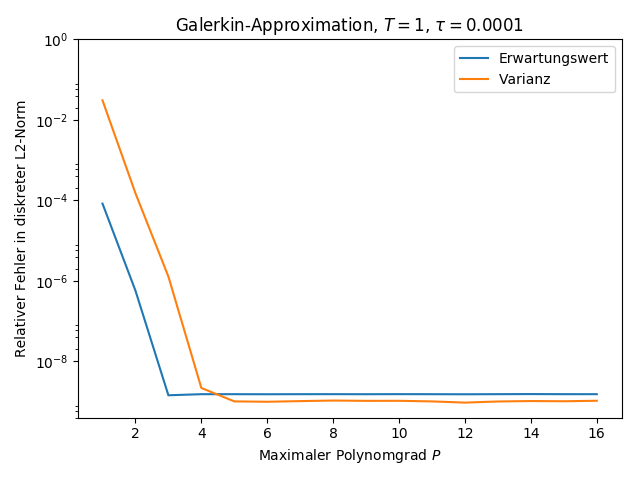
\includegraphics[width=\linewidth]{Figures/galerkin_bydegree_trial1_t1.png}
\endminipage
\minipage{0.5\textwidth}
  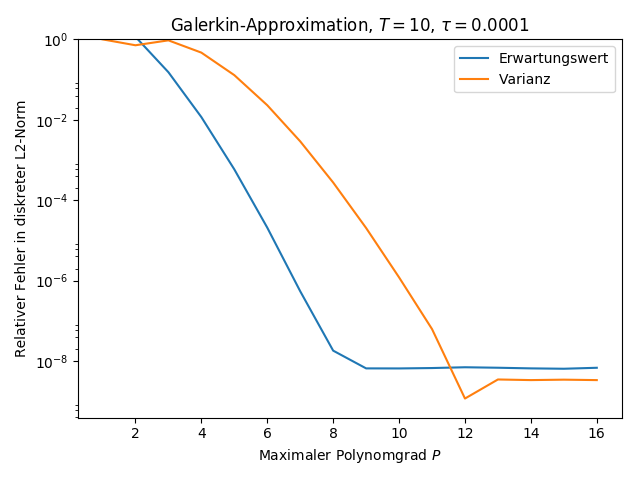
\includegraphics[width=\linewidth]{Figures/galerkin_bydegree_trial1_t10.png}
\endminipage
  \caption{Approximation des Erwartungswert und der Varianz von \nameref{trial:1} zu fixen Zeitpunkten durch Galerkin-Ansatz mit $\tau=0.0001$ und verschiedenen Polynomgraden.}
  \label{fig:galerkin_bydegree_trial1}
\end{figure}
\newline
Anschließend beobachten wir in Abbildung \ref{fig:galerkin_bystoptime_trial1} das Verhalten für wachsende Stoppzeit $T$, ebenfalls anhand der einfachen \nameref{trial:1}. Die Parameter für die Quadratur sind dabei hoch genug gewählt um als relevante Fehlerquellen ausgeschlossen werden zu können. Die Wahl $P=25$ schließt, begründet durch die Beobachtungen aus Abbildung \ref{fig:galerkin_bydegree_trial1}, den Einfluss des Polynomgrads als Fehlerquelle für die Zeitspanne $T\le 10$ aus.\\
Wir erkennen, dass im linken Fall der niedrige Polynomgrad mit $P=5$ dafür sorgt, dass die Approximationen ab $T=1$ zunehmend schlechter werden. Im rechten Fall mit $P=25$ ist keine Verschlechterung der Fehler im Erwartungswert und Varianz zu beobachten. Der Fourier-Fehler im Sinne von Satz \ref{th:adapted22} hingegen zeigt einen gewissen Aufwärtstrend bezüglich der Zeit $T$.
\begin{figure}[!htb]
\minipage{0.55\textwidth}
  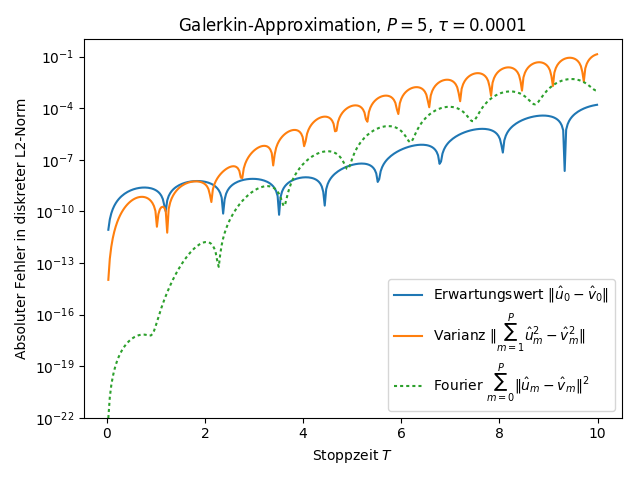
\includegraphics[width=\linewidth]{Figures/galerkin_bystoptime_trial1_fixeddegree5.png}
\endminipage
\minipage{0.55\textwidth}
  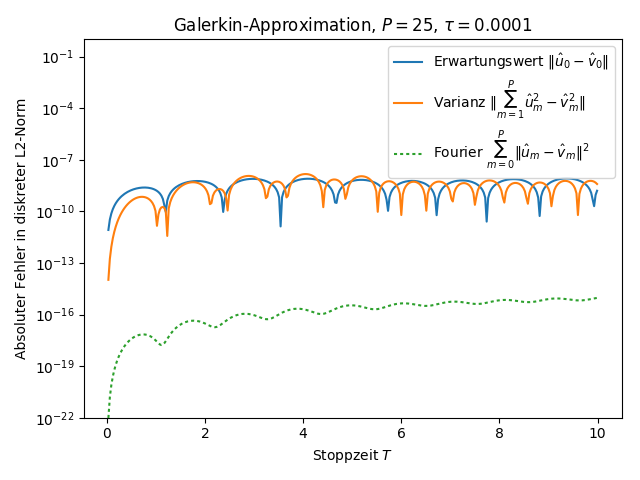
\includegraphics[width=\linewidth]{Figures/galerkin_bystoptime_trial1_fixeddegree25.png}
\endminipage
  \caption{Verschiedene Fehler von \nameref{trial:1} mit fixem Polynomgrad und hinreichend guter Quadraturformel.}
  \label{fig:galerkin_bystoptime_trial1}
\end{figure}
\newline
In Abbildung \ref{fig:galerkin_bystoptime_trial3}, welche die Fehler der eindimensionalen \nameref{trial:3} mit $Y\sim\mathcal{U}(10,50)$, beobachten wir zusätzlich auch einen leichten Aufwärtstrend der Fehler des Erwartungswerts und der Varianz bezüglich der Zeit $T$.
\begin{figure}[!htb]
\centering
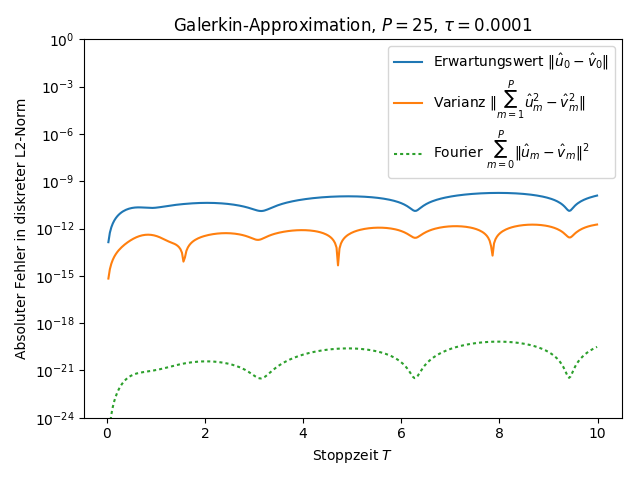
\includegraphics[width=0.75\linewidth]{Figures/galerkin_bystoptime_trial3_fixeddegree25_big.png}
\caption{Verschiedene Fehler von \nameref{trial:3} mit fixem Polynomgrad und hinreichend guter Quadraturformel.}
\label{fig:galerkin_bystoptime_trial3}
\end{figure}
\todo[inline]{Problem4: Es ist nicht ganz klar, was eigentlich rauskommen soll. Durch fehlende Referenzlösungen für die Varianz an vielen verschiedenen Zeitpunkten ist es schwierig, beliebige Beispiele (insbesondere mehrdimensionale) zu beobachten.}